\documentclass[11pt]{article}
\usepackage[T1]{fontenc}
\usepackage{lmodern,microtype}
\usepackage[a4paper,margin=24mm]{geometry}
\usepackage{amsmath,amssymb,graphicx,booktabs,array,xcolor}
\usepackage[colorlinks=true,urlcolor=blue!45!black]{hyperref}
\hypersetup{pdftitle={Why centering helps a random matching},pdfsubject={An illustrated reading guide for problem 21}}
\usepackage{enumitem}
\setlist{itemsep=5pt,topsep=6pt}
\definecolor{ink}{HTML}{26394B}
\definecolor{teal}{HTML}{176B8A}
\definecolor{rust}{HTML}{BB5B28}
\newcommand{\E}{\mathbb E}
\newcommand{\shc}{\operatorname{sinhc}}
\newcommand{\pagetitle}[2]{\noindent{\small\sffamily\color{teal}#1}\par\vspace{5pt}\noindent{\LARGE\bfseries\color{ink}#2}\par\vspace{12pt}}
\setlength{\parindent}{0pt}
\setlength{\parskip}{7pt}
\begin{document}
\pagetitle{PROBLEM 21 / READING GUIDE}{Why centering helps a random matching}

A permutation matrix records a random one-to-one matching. Every row and every column contains exactly one entry equal to one. All other entries are zero.

Subtracting the mean $1/N$ from an entry is called \emph{centering}. The question is what happens when we multiply many such entries and take the expectation. This is the small probabilistic calculation hidden inside much larger spectral-gap proofs.

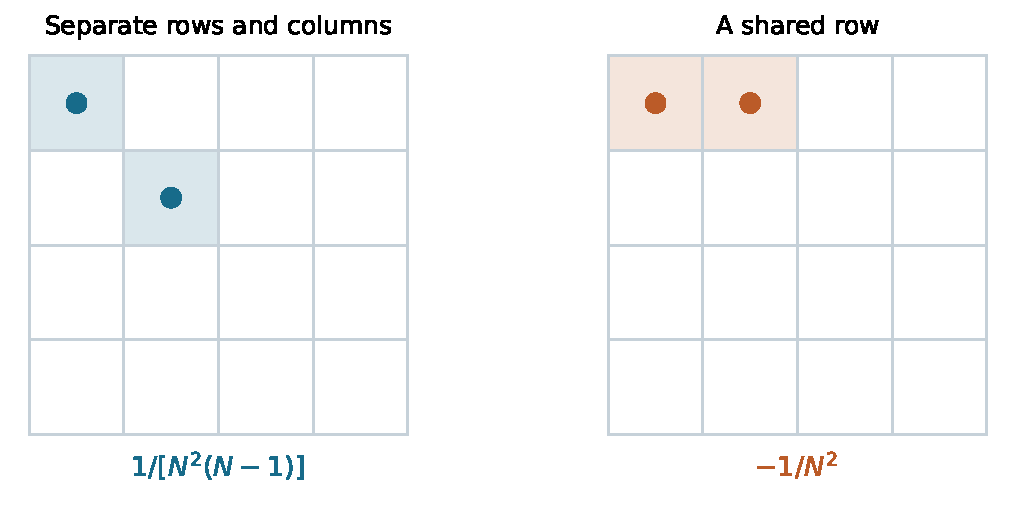
\includegraphics[width=\textwidth]{../figures/cell-patterns.pdf}

The dots show the two requested cells, not a realized permutation. For cells in different rows and columns,
\[
\E[(M_{11}-1/N)(M_{22}-1/N)]
=\frac1{N(N-1)}-\frac1{N^2}
=\frac1{N^2(N-1)}.
\]
For cells sharing a row, both indicators cannot equal one. Their centered product instead has expectation $-1/N^2$.

\textbf{The lesson.} Separate cells gain an extra factor of about $1/N$. Conflicting cells do not. Taking absolute values before evaluating the product would hide this cancellation.

\textbf{What the manuscript adds.} A direct proof handles arbitrary mixed products, including repeated cells and independent matching colors. It gives an exact attained maximum when there are zero or one conflicting centered singletons. For distinct diagonal cells, we determine the first transition, a hierarchy of later corrections, and the sharp first error. One formula covers every permitted order.

The known starting recurrence and leading terms are credited to Collins and Nagatsu. The graph application is the estimate in Bordenave's Proposition 28, imported by Brito, Dumitriu and Harris.

\newpage
\pagetitle{THE PROOF IN THREE MOVES}{Preserve cancellation until it has paid off}

Call a requested cell \emph{isolated} if no other requested cell of the same color shares its row or column. An isolated centered singleton appears once, centered, and with no uncentered copy of that cell.

\textbf{1. Set those singletons aside.} Every other cell factor is an affine expression $c+dM$, because an indicator satisfies $M^2=M$. Expanding these factors selects some matches that must occur.

\textbf{2. Condition only on compatible matches.} If $r$ selected matches have distinct rows and columns, they occur with probability $1/(N)_r$. Delete their rows and columns. The remainder is exactly a uniform permutation of size $N-r$.

The original centering is still $1/N$. For the remaining matrix $U$, set $Z=NU-1$. Every remaining row now sums to $r$. It does not sum to zero.

\textbf{3. Sum a row before taking absolute values.} Let $\mu_j$ be the expectation of the product of $j$ separated $Z$ entries. The row sum gives
\[
(N-r-j+1)\mu_j
=(r+2j-2)\mu_{j-1}+(j-1)\mu_{j-2}.
\]
For $j=1$, omit the last term. The initial values are $\mu_0=1$ and $\mu_1=r/(N-r)$ for $r<N$. Full depletion uses only the empty product $\mu_0$. All coefficients are nonnegative.

A new column keeps all $j$ factors. A used column collides with an old factor, and the identity
\[
Z_uZ_v=-Z_u-Z_v-1
\]
removes one or two factors. This turns a cancellation problem into a positive recurrence we can bound by induction.

\textbf{The resulting estimate.} For $a$ distinct cells, $h$ isolated centered singletons and $b$ conflicting centered singletons,
\[
|\E P|\le\sqrt e\,2^bN^{-a}
\left(\frac{\sqrt{a-1}}{\sqrt N-\sqrt{a-1}}\right)^h,
\qquad 2\le a\le\sqrt N.
\]
Each isolated singleton earns an additional small factor. The exact theorem retains the full depleted moment instead of bounding it geometrically. The next page explains the resulting maximum. Compatible uncentered matches with $N=a^2$ show why the universal prefactor in the displayed scalar estimate cannot be smaller than $\sqrt e$.

\textbf{Why the conditioning matters.} Exposing both an image and a preimage can reveal two arrows. For a permutation of four elements, knowing $2\mapsto3$ and $4\mapsto2$ leaves two choices for the image of row 1. Counting only one removed arrow would give the wrong denominator. The manuscript records this source-proof issue precisely and supplies the replacement argument above.

\newpage
\pagetitle{THE SHARP MIXED BOUND}{Sharp bounds with explicit attaining patterns}

Fix the dimension $N$, the number $a\le N$ of distinct requested cells, and the number $h$ of isolated centered singletons. Allow arbitrary repeated powers and any number of independent permutation colors.

\textbf{When there is no conflicting centered singleton, the maximum is attained by one simple pattern:} choose $a$ cells in distinct rows and columns of a single permutation, center $h$ of them, and leave the other $r=a-h$ raw.

The exact largest absolute expectation is
\[
\boxed{\frac{N^{-h}\mathcal P_h(N,a-h)}{(N)_a}.}
\]
The polynomial has positive coefficients. Its first values are
\[
\mathcal P_0(N,r)=1,\qquad
\mathcal P_1(N,r)=r,\qquad
\mathcal P_2(N,r)=r^2+r+N.
\]
In general, partition the $h$ labeled centered factors into blocks. A block of size $j$ carries weight $((j-1)N+r)(j-1)!$. Add the products of these weights over all partitions. This is a finite recipe for $\mathcal P_h$.

\textbf{Why this is the maximum.} Compatible conditioning produces exactly this polynomial divided by a falling factorial. Its block weights increase when more matches are prescribed. Two separate colors can be merged into one larger positive partition sum. The affine weights of repeated cells are at most one. Each step gives an upper bound, and the compatible pattern above makes the final bound an equality.

\textbf{One conflicting centered singleton also has an exact maximum.} Here $h\le a-2$, and the answer is
\[
\boxed{\frac{N^{-h-1}\mathcal P_h(N,a-h-1)}{(N)_{a-1}}.}
\]
Choose a centered cell sharing a row with a raw cell. Keep the other requested cells compatible with the raw support and away from that centered cell. The raw match forces its indicator to zero, contributing exactly $-1/N$. The remaining factors give the displayed depleted moment. For $b\ge1$, multiplying this second expression by $2^{b-1}$ gives a valid general bound. Attainment is asserted only for $b=1$.

\textbf{One isolated centered singleton makes the gain concrete.} When $b=0$, $h=1$ and $a\ge2$, the exact maximum is
\[
\frac{a-1}{N(N)_a}.
\]
After prescribing $a-1$ raw matches, the remaining centered factor has scaled conditional mean $(a-1)/(N-a+1)$. At $N=a^2$, this is about $1/a$. The earlier geometric factor is about $1/\sqrt a$, so the exact calculation improves this full product bound by a factor of order $\sqrt a$.

\textbf{The improvement depends on composition.} With fixed $h$, the gain at $N=a^2$ has order $a^{h/2}$. When all $a$ factors are centered and $a$ grows, pair partitions show that the square-root singleton scale remains necessary. The theorem distinguishes these regimes instead of assigning the same loss to every product.

\newpage
\pagetitle{THE FIRST TRANSITION}{Why the order enters as a cube}

For $k$ distinct diagonal cells define
\[
a_k(N)=\E\prod_{i=1}^k(M_{ii}-1/N),\qquad R_k=a_k/L_k.
\]
The known leading terms depend on parity:
\[
L_{2m}=(2m-1)!!N^{-3m},\qquad
L_{2m+1}=\frac{4m}{3}(2m+1)!!N^{-3m-2}.
\]
We use $k\ge2$. The first centered moment is zero and has no such ratio.

The normalized even recurrence changes by order $m^2/N$ at step $m$. There are about $m$ steps, so the accumulated change has scale $m^3/N$. The odd recurrence averages these changes differently, which explains the two limits.

The proof turns that intuition into bounds:
\[
R_k-1\ge\frac{2k^3}{27N}\quad(2\le k\le N),\qquad
R_k\le e^{3k^3/N}\quad(2k\le N).
\]
Thus $R_k\to1$ \textbf{exactly when} $k^3/N\to0$. This settles the optimal-scale question posed in the published paper by Collins and Nagatsu.

At $k^3/N\to c$, the even and odd ratios tend to
\[
\cosh\left(\frac23\sqrt c\right),\qquad
\frac{\sinh(\frac23\sqrt c)}{\frac23\sqrt c}.
\]
The second value is interpreted as one at $c=0$. For $c=9/4$, the limits are about $1.543$ and $1.175$. The original leading term is no longer relatively accurate, and parity remains visible.

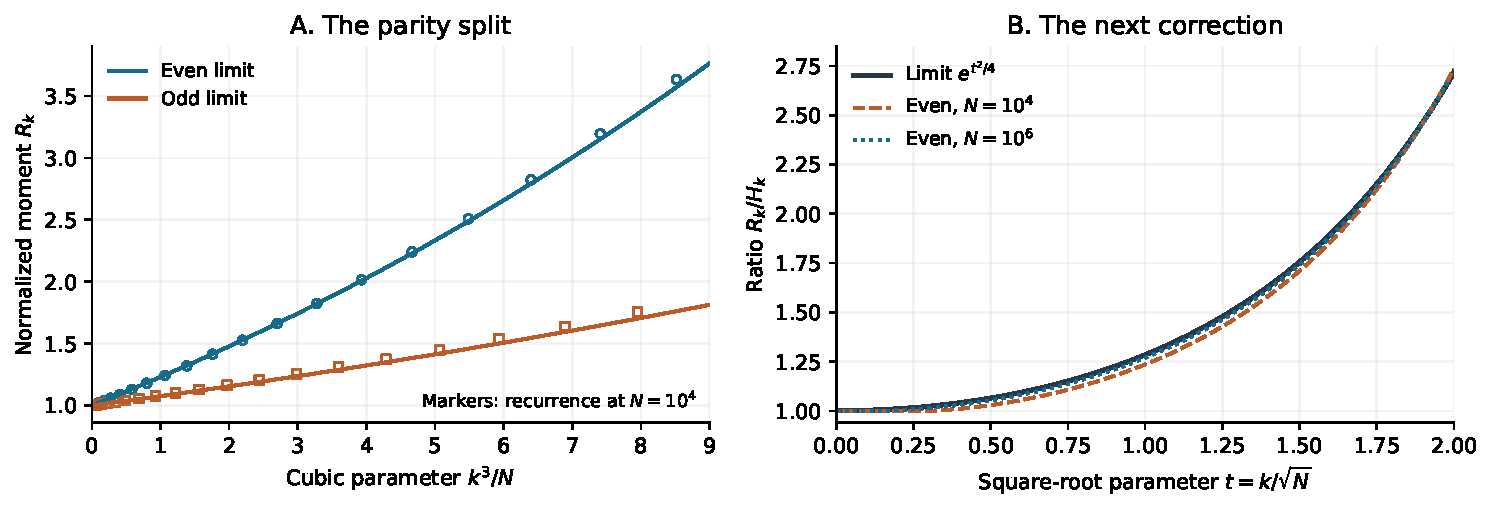
\includegraphics[width=\textwidth]{../figures/moment-regimes.pdf}

Left: the critical transition. Right: a later correction described on the next page. Markers and finite-size curves come from the positive recurrence. They illustrate the theorems rather than prove them.

\newpage
\pagetitle{THE NEW EXTENSION}{Pairs, triples and the next boundary}

Clear the denominators by setting $Q_k=(N)_kN^ka_k$. Its positive generating function is
\[
\sum_{k\ge0}Q_k\frac{z^k}{k!}
=\exp\left(N\sum_{j\ge2}\frac{j-1}{j}z^j\right).
\]
As a formal series this is a classical Laguerre identity. For the permutation application, $k\le N$. Its coefficients count weighted partitions of the $k$ labeled factors. There are no singleton blocks.

A block of size $j$ carries weight $N(j-1)(j-1)!$. A pair therefore has weight $N$, a triple has weight $4N$, and a block of four has weight $18N$.

For six factors the complete count is
\begin{center}
\begin{tabular}{llr}
\toprule
Partition shape & Number and weight & Contribution\\
\midrule
Three pairs & $15$ partitions, each $N^3$ & $15N^3$\\
Two triples & $10$ partitions, each $16N^2$ & $160N^2$\\
A pair and a block of four & $15$ partitions, each $18N^2$ & $270N^2$\\
One block of six & $1$ partition of weight $600N$ & $600N$\\
\bottomrule
\end{tabular}
\end{center}
So $Q_6=15N^3+430N^2+600N$.

\textbf{Pairs give the leading term.} The leading even contribution uses pairs only. The leading odd contribution uses one triple and otherwise pairs. Extra triples arrive with an even or odd parity restriction. Their exponential sums are precisely a hyperbolic cosine and a normalized hyperbolic sine.

Set $K=2\lfloor k/2\rfloor$, $\lambda=\frac23\sqrt{K^3/N}$ and
\[
H_k=\cosh\lambda\ \ (k\text{ even}),\qquad
H_k=\sinh\lambda/\lambda\ \ (k\text{ odd}).
\]
The extended theorem proves $R_k/H_k\to1$ throughout $k=o(\sqrt N)$. This includes orders much larger than $N^{1/3}$, where $R_k$ itself already diverges.

\textbf{Blocks of four mark the next boundary.} When $k^2/N\to d>0$, their contribution survives. The triples use a vanishing fraction of the labels, but their cumulative effect on the number of available pairings stays nonzero. Combining these effects with the permutation probability gives
\[
\frac{R_k}{H_k}\longrightarrow e^{d/4}.
\]
At $k\sim\sqrt N$, the correction is $e^{1/4}\approx1.284$. Including the factor $e^{k^2/(4N)}$ restores relative accuracy beyond bounded square-root ranges, all the way to $k=o(N^{3/5})$. The next page explains this further boundary and the first error.

\newpage
\pagetitle{THE CORRECTION HIERARCHY}{Every retained exponent extends the range}

The compact formula is
\[
R_k\sim H_k\exp\{NG(\sqrt{k/N})\},\qquad
G(t)=\sum_{j\ge4}\frac{2t^j}{j(j-2)}.
\]
It is uniformly accurate throughout every range $2\le k\le b_N=o(N)$. Expanding its exponent gives
\[
NG(\sqrt{k/N})
=\frac{k^2}{4N}+\frac{2k^{5/2}}{15N^{3/2}}+\frac{k^3}{12N^2}+\cdots.
\]
Each first omitted term identifies the next boundary. The following approximations are for $R_k$, and the windows are sharp within the sublinear range.

\begin{center}
\begin{tabular}{ll}
\toprule
Approximation & Relative-accuracy window\\
\midrule
$1$ & $k=o(N^{1/3})$\\
$H_k$ & $k=o(N^{1/2})$\\
$H_ke^{k^2/(4N)}$ & $k=o(N^{3/5})$\\
$H_ke^{k^2/(4N)+2k^{5/2}/(15N^{3/2})}$ & $k=o(N^{2/3})$\\
\bottomrule
\end{tabular}
\end{center}

Put $W_{N,k}=R_k/[H_ke^{k^2/(4N)}]$. At $k\sim\sqrt N$,
\[
N^{1/4}(W_{N,k}-1)\longrightarrow
\begin{cases}-11/30,&k\text{ even},\\19/30,&k\text{ odd}.
\end{cases}
\]
Thus the $N^{-1/4}$ error rate cannot be improved uniformly on this range. More generally, the exact asymptotic worst-case constant on $k\le C\sqrt N$ is $\sqrt C/2+2C^{5/2}/15$.

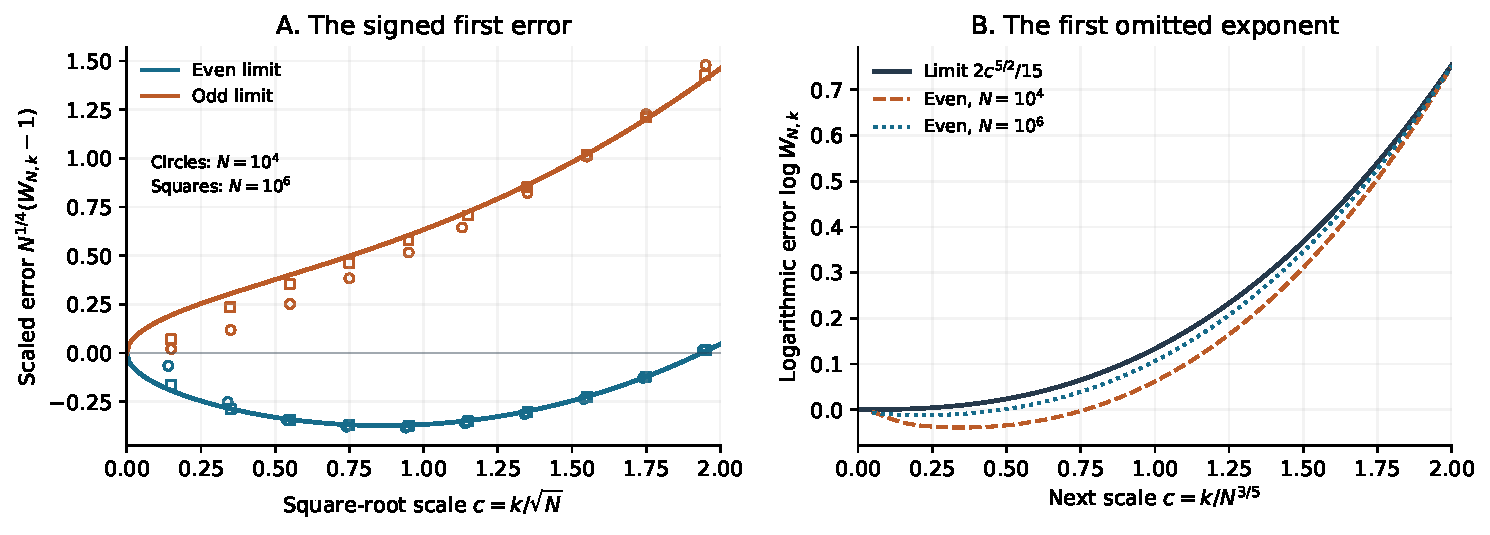
\includegraphics[width=\textwidth]{../figures/rate-and-hierarchy.pdf}

Left: the signed first error at square-root scales. Right: the first omitted exponent at $k\sim cN^{3/5}$. Recurrence values corroborate the proved limits. Keeping the falling factorial $(N)_k$ exact gives the further formula on the next page.


\newpage
\pagetitle{A FORMULA AT EVERY ORDER}{The largest remaining error occurs at cubic orders}

The previous page used the short correction $H_ke^{k^2/(4N)}$. A fuller formula keeps the exact permutation denominator and the parity amplitude. Put $\epsilon=k\bmod2$, $K=k-\epsilon$, $x=\sqrt{K/N}$ and
\[
q(x)=x+(x^2-1)\log(1+x)-\frac{x^2}{2}-\frac{2x^3}{3}.
\]
The approximation for $R_k$ is
\[
\boxed{\mathcal A_{N,k}
=\frac{N^k}{(N)_k}H_k e^{Nq(x)}(1+x)^{\epsilon-1/2}.}
\]
All factors are positive and finite for every $2\le k\le N$. Retaining $(N)_k$ makes the formula valid even at the top order $k=N$.

\textbf{The optimal error is explicit.} The theorem proves
\[
\sup_{2\le k\le N}\left|\frac{R_k}{\mathcal A_{N,k}}-1\right|
=C_*N^{-1/3}+o(N^{-1/3}),\qquad C_*\approx0.39549627.
\]
This is an asymptotic equality, not a finite-$N$ upper bound with that constant. Odd orders near $1.1654N^{1/3}$ attain the largest limiting error. At those orders the approximation is slightly too large. The even error has the opposite sign and a smaller maximum.

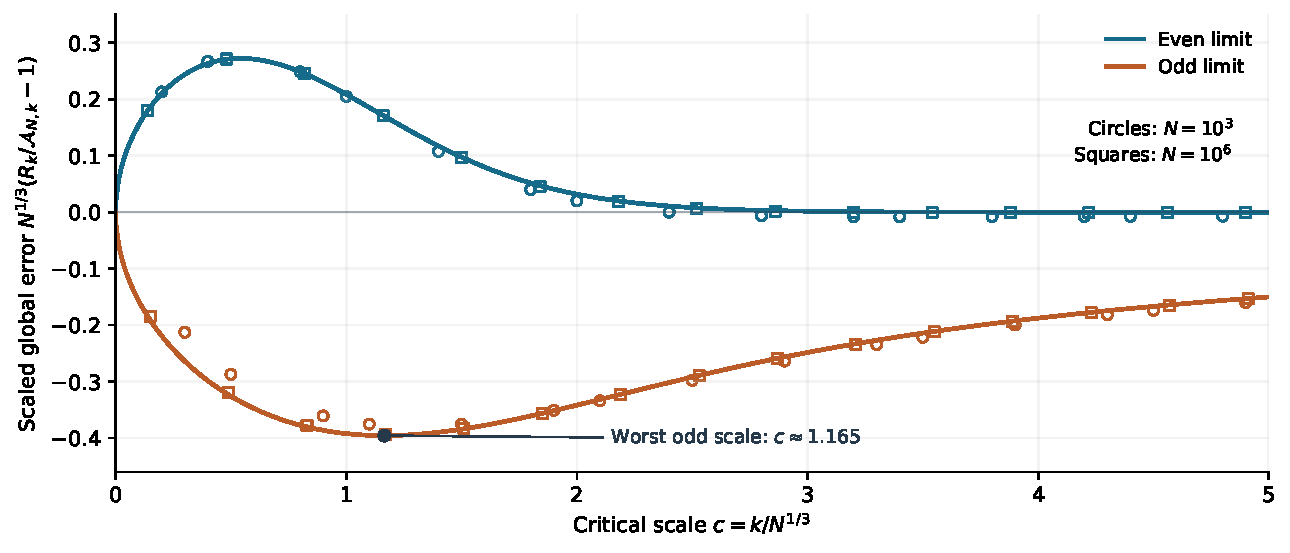
\includegraphics[width=\textwidth]{../figures/global-error.pdf}

The horizontal coordinate is $c=k/N^{1/3}$. The curves are the proved limits of $N^{1/3}(R_k/\mathcal A_{N,k}-1)$. Markers come from exact recurrence values. The proof controls both small and large $c$, so the conclusion covers all orders, not only those visible in the plot.

\textbf{Why another correction helps.} Pair and four-block effects cancel against the retained exponent. What remains measures the difference between the mean triple count with a parity restriction and the unrestricted mean. At much larger orders the two means are nearly equal. This explains why the largest error returns to the cubic scale.

\textbf{Two rates, two formulas.} The $N^{-1/4}$ rate on the previous page is optimal for the shorter approximation on square-root ranges. The $N^{-1/3}$ rate here is optimal for the displayed fuller approximation on the entire range. Both claims concern their specified formulas.

\newpage
\pagetitle{BACK TO GRAPHS}{What this proves for the spectral argument}

\textbf{Random lifts.} Each base edge carries an independent random permutation. Orient the base edges once, and treat each permutation as a color. The mixed-product theorem directly supplies Bordenave's Proposition 28.

\textbf{Biregular graphs.} Match the left half-edges to the right half-edges. There are
\[
L=n_Ld_L=n_Rd_R
\]
half-edges on each side, so the random block is a permutation matrix of size $L$. Its entries are centered at $1/L$. This is the input used by Brito, Dumitriu and Harris in preprint Lemma 7, published as Lemma 5.6.

\textbf{The proof chain.}
\begin{enumerate}
\item Expand powers of a non-backtracking matrix into walks that do not immediately reverse an edge.
\item Expand a high norm moment into products of matching entries.
\item Apply the mixed-product bound to each fixed pattern.
\item Count the patterns and control the contribution of local tangles.
\item Translate the non-backtracking bound back to adjacency eigenvalues.
\end{enumerate}
The manuscript proves the probability estimate in step 3 and explains the surrounding chain. The graph enumeration and tangle remainder are separate requirements.

\textbf{A concrete spectral bridge.} If the degrees are $d_L,d_R\ge2$, put $\alpha=d_L-1$ and $\gamma=d_R-1$. A positive adjacency singular value $s$ and the associated non-backtracking parameter satisfy
\[
s^2=x+\frac{\alpha\gamma}{x}+\alpha+\gamma,\qquad x=z^2.
\]
The circle $|x|=\sqrt{\alpha\gamma}$ corresponds to
\[
|\sqrt\alpha-\sqrt\gamma|\le s\le\sqrt\alpha+\sqrt\gamma.
\]
An $s$ above the upper endpoint forces a non-backtracking root outside the circle. This is why controlling those roots yields a spectral gap.

\textbf{What remains separate.} The sharper moment formulas do not automatically give a better graph eigenvalue bound. The proof does not certify every later step in the cited graph papers. Classical asymptotic methods provide another route to the diagonal corrections. The attained mixed maximum is a distinct contribution candidate, with historical priority still subject to a bounded literature assessment.

\vfill
{\small\color{ink}\textbf{Reading route.} Start with manuscript Sections 2 and 8 for the requested estimate and graph application. Sections 3 through 7 give the asymptotic results, with explicit finite rate constants in Appendix A and the full-range sharp-error proof in Appendix B. Section 9 checks published equation (62), page 1428. Primary sources: \href{https://smf.emath.fr/download/pdf/1498332}{Bordenave, Proposition 28, page 1426}, \href{https://arxiv.org/abs/1804.07808v6}{Brito, Dumitriu and Harris, Lemma 7}, and \href{https://doi.org/10.5802/alco.480}{Collins and Nagatsu, Proposition 3.3 and Remarks 3.4 and 3.5}.}
\end{document}
